\begin{figure}[h]
	\centering
	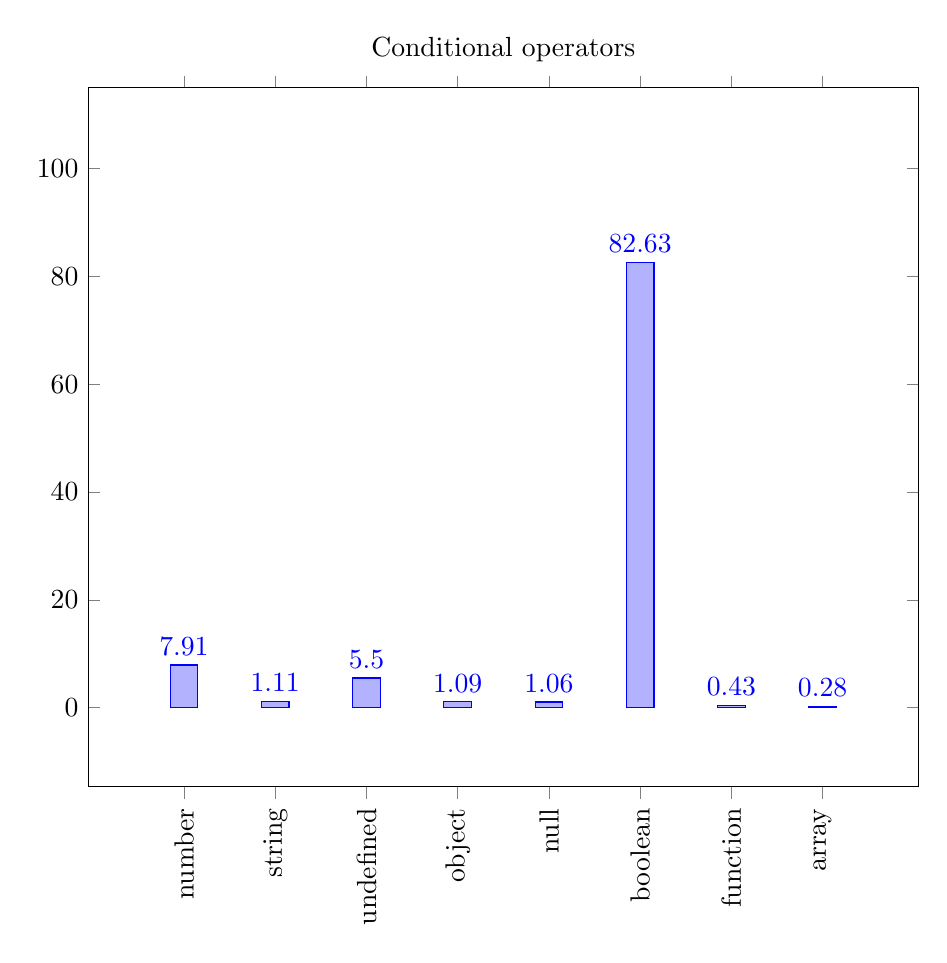
\begin{tikzpicture}
		\begin{axis}[
			ybar,
			title=Conditional operators,
			width=1\textwidth,
			ybar=0pt,
			ymax=100,
			enlargelimits=0.15,
			legend style={at={(0.5,-0.2)}, anchor=north,legend columns=-1},
			symbolic x coords={number,string,undefined,object,null,boolean,function,array},
			xtick=data,
			nodes near coords, 
			nodes near coords align={vertical},
			x tick label style={rotate=90,anchor=east},
		]
		\addplot coordinates {
			(number, 7.91)
			(string, 1.11)
			(undefined, 5.50)
			(object, 1.09)
			(null, 1.06)
			(boolean, 82.63)
			(function, 0.43)
			(array, 0.28)
		};
		\end{axis}
	\end{tikzpicture}
	\caption[Conditional operators]{\textbf{Type distribution for conditional operators} - It includes all operators that trigger a condition check before branching: ${if-then-else}$, ${switch-case}$, ${while}$, ${for}$, ${||}$, ${\&\&}$, ${ ? : }$.
	}
\end{figure}